\documentclass[]{usiinfbachelorproject}

\usepackage{float}
\usepackage{subcaption}
\usepackage{graphicx}
\usepackage{chngcntr}
\usepackage{xcolor}
\usepackage[colorinlistoftodos,prependcaption,textsize=tiny]{todonotes}

\counterwithin{figure}{section}

\captionsetup{labelfont={bf}}

\author{Andrea Vicari}
\newcommand{\applicationName}{Smart--IVC}
\newcommand{\cfbox}[2]{%
    \colorlet{currentcolor}{.}%
    {\color{#1}%
    \fbox{\color{currentcolor}#2}}%
}
\title{\applicationName}
\subtitle{Enhanced Visualization of Cities Through Smart Visual Queries}
\versiondate{\today}
\begin{committee}
%With more than 1 advisor an error is raised...: only 1 advisor is allowed!
\advisor[Universit\`a della Svizzera Italiana, Switzerland]{Prof.}{Michele}{Lanza}
%You can comment out  these lines if you don't have any assistant
\assistant[Universit\`a della Svizzera Italiana, Switzerland]{Dr.}{Andrea}{Mocci}
\end{committee}


\abstract {Cities constantly evolve, with the appearance of new neighborhoods and the disappearance of old buildings. Information about cities are nowadays stored as static data inside huge storages where it is difficult and slow to retrieve particular information. Moreover, different data sources about cities are not aggregated since they are provided by both public websites on the Internet and by public sectors of the city.\\

A visualization can help supporting any decision that involves city evolution,  especially in the contest of what is called a Smart City. No such service exists that provides a unique environment in which the user can both visualize a city and interact with its elements. The only technologies available are either not exhaustive or too complex to use. For example, it is possible to find technologies online that are limited to provide a 3D--visualization without any kind of interaction between the map and the user.\\

\applicationName\ provides an interactive 3D--visualization  model of cities,  integrating heterogeneous data, and supporting complex visual queries. \applicationName\ is  an application accessible by everyone (since it is both user--friendly and publicly available) and that aims to enhance the city visualization, getting closer to the user needs.

%Web users have to aggregate different data from various sources whenever they are looking for some information on the Internet. Think about the student who is looking for a rented room near her university: she firstly uses a specific website to find the advertisement of a room for rent, she then looks for the address on another website that provides a map service to see if the house is located where she desires.\\
%
%No such service exists that provides a unique environment in which the user can both visualize a city and interact with its elements. The only technologies available are either not exhaustive or too complex to use.\\
%
%This thesis introduces \applicationName\ a web application that provides an intuitive interface and prevents the user from jumping from website to website. Through the form of a 3D-environment, this application provides an interactive visualisation of cities in which the user can directly “communicate” with the elements, executing queries on them. After having clicked on a building in the map, the user is able to get information (coordinates, address, floors etc.) about that construction and also find out what are the various relations between that specific building and the other entities in the city.\\
}

\begin{document}
\maketitle
\thispagestyle{empty}
\tableofcontents
\newpage
\thispagestyle{empty}
\listoffigures
%\listoftables
\newpage
%%%%%%%%%%%%%%%%%%%%%%%%%
%%%%%%%%%%%%%%%%%%%%%%%%%
\section{Introduction} \label{introduction}
%%%%%%%%%%%%%%%%%%%%%%%%%
Cities nowadays are in constant evolution. They change their structure over time through the appearance of new entities and the disappearance of old ones, thus they are very unsteady and prone to changes. Important changes might be considered with regard to the deployment and management of all types of infrastructures within cities. For example, the decision of which building to demolish in order to make space for the construction of a new mall in a city.\\

Moreover, cities have a very large impact on the economic and social development of nations: they represent the real foundation where people live, where companies have their business and in which numerous services are provided. Often, a city overview is not available, so decision may be taken without having a big picture of the surrounding environment. This could lead to choices that might have a negative impact on the current city, reducing the efficiency and the life quality of the citizens. Also, data is not very well aggregated since different information about the same city can be provided by different public and online services for example Google and OpenStreetMap or by public city entities like the cadastre office.\\

To control these changes and to aggregate this data, a visualization, which provides a city overview, is required. Such a visualization is considered to be the first step towards what it is called a Smart City. A Smart City can be defined as a city which uses information and communication technologies so that its critical infrastructure as well as its components and public services provided are more interactive, efficient and so that citizens can be made more aware of them.\\

\subsection{Contributions}
\applicationName\ aims to solve the problem generated by the static and non--aggregated nature of data regarding cities (as mentioned above) through an Interactive 3D--Visualization model. Therefore, the main contributions that \applicationName\ provides are:
\begin{itemize}
	\item The visualization of a 3D city model. As a use case for this Bachelor Project, the city of Lugano has been taken into account.
	\item The interactivity that the user has with the entities inside the city: buildings can be clicked in order to receive information about them and in order to receive information between the selected building itself and the rest of the entities in the city.
	\item The possibility to have a graphical city overview using a very intuitive system of visual queries which produce results that are immediately visible through the highlighting or colouring of the buildings. 
\end{itemize} 
\subsection{Structure of the report}
\begin{itemize}
	\item {\bf Chapter 2} discusses the state of the art. It talks about already existing tools which allow city visualization in a virtual environment. In particular, it focuses on tools that use the Cesium framework comparing and contrasting the existing features with the ones proposed in \applicationName.
	\item {\bf Chapter 3} is the main chapter of the entire report. It shows how \applicationName\ has been developed step by step. The decisions that have been taken and the technologies adopted will be explained and discussed in detail starting from the parsing of the unique .xml file provided by the Comune of Lugano and ending with the final result (i.e., the 3D--visualization of the entire city). 
	\item {\bf Chapter 4} illustrates showing some use cases of the application. Examples will be illustrated and explained in detail, in order to show the features proposed by \applicationName. 
	\item {\bf Chapter 5} is the conclusion of this report. Here, the current limitations of the application will be presented. Finally, we will discuss and analyze the future work and the different paths that \applicationName\ might take.
\end{itemize}
%%%%%%%%%%%%%%%%%%%%%%%%%
%%%%%%%%%%%%%%%%%%%%%%%%%
\section{State of the Art} \label{stateOfTheArt}
%%%%%%%%%%%%%%%%%%%%%%%%%
As explained above, city visualization is a subject undergoing intense study, therefore there can found new projects about it everyday, on the Internet. Still, the uniqueness of \applicationName\ resides on the fact that it provides, not only a visualization of a city but, above all, it gives the user the possibility to interact with the city itself through a simple system of visual queries.\\

Before getting into the details with \applicationName, the current state of city visualization must be clarified and, since the projects about this topic are so various and so many, in this Chapter, the ones that relate most with the final outcome of this Bachelor Project will be presented.\\

At first, some 3D--city--model based on OpenStreetMap data will be presented, as {\bf OSMBuildings}, {\bf F4 Map} and {\bf ViziCities}. Then, the {\bf Cesium framework} will be introduced, since it has been used used as a basis for \applicationName. At the end, the work done by the {\bf Swiss Geospatial Portal} (still using Cesium), will be analyzed and compared with the application described in this report. 
\subsection{OpenStreetMap--Based Frameworks}
OpenStreetMap, is a project that creates and distributes free geographic data for the world. In the last period, the third dimension has become a growing topic at OSM, so it is now possible to add detailed buildings and a lot of minor objects. Here, some of the frameworks that use this data, will be analyzed.
\subsubsection{OSMBuildings}
OSMBuildings is an engine for displaying 3D buildings on a web map. It uses information on buildings provided by OpenStreetMap and it renders them on a map layer.\\Altough in some cases, buildings are very detailed (i.e., in big cities like New York or Berlin), it does only provide a visualization without any kind of interaction.
\begin{figure} [H]
\centering
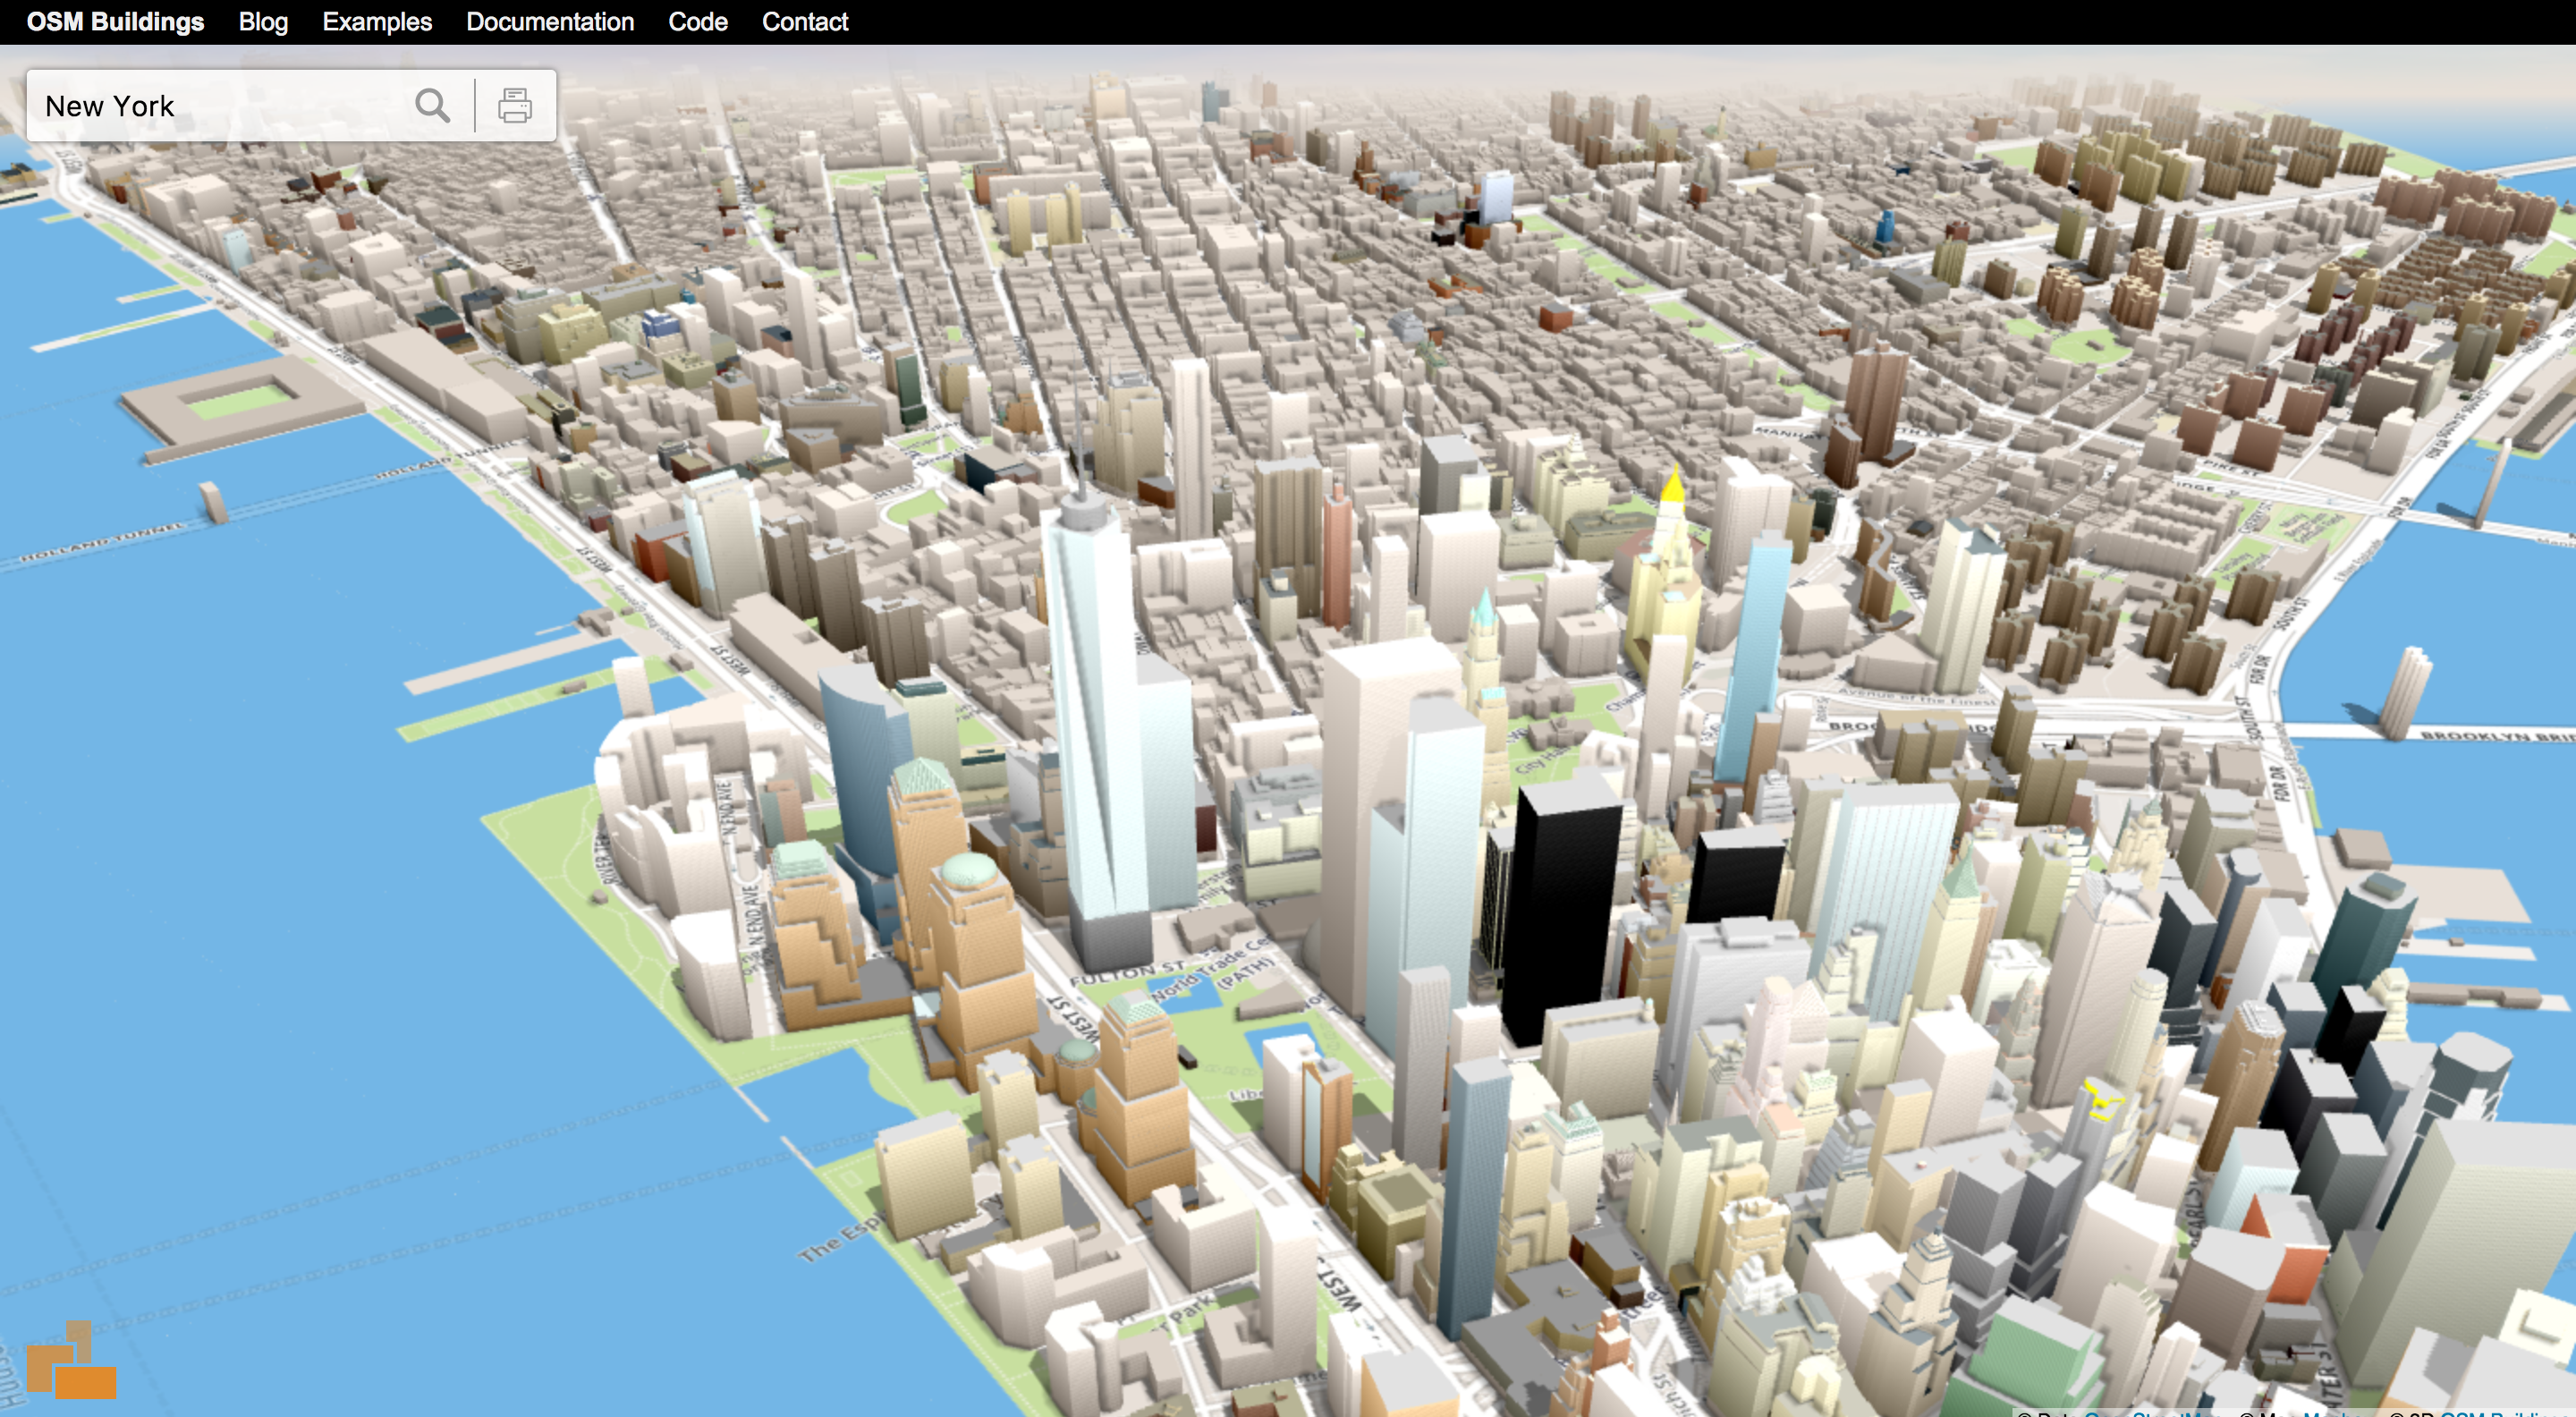
\includegraphics[width=0.8\textwidth]{chapter2/images/OSM_Building}
\caption{A visualization of New York city using OSMBuildings}
\label{fig:OSM_Building}
\end{figure}

\subsubsection{F4 Map}
The F4 Map is an OSM-based 3D map using the WebGL technology. Also this map, uses Open Street Map's buildings but also adds some non--OSM--provided features like trees, cranes and other data.\\
 Some 3D models are used (not based on buildings data in OpenStreetMap) for some specific buildings (e.g. the Eiffel Tower in the example below).
\begin{figure}[H]
\centering
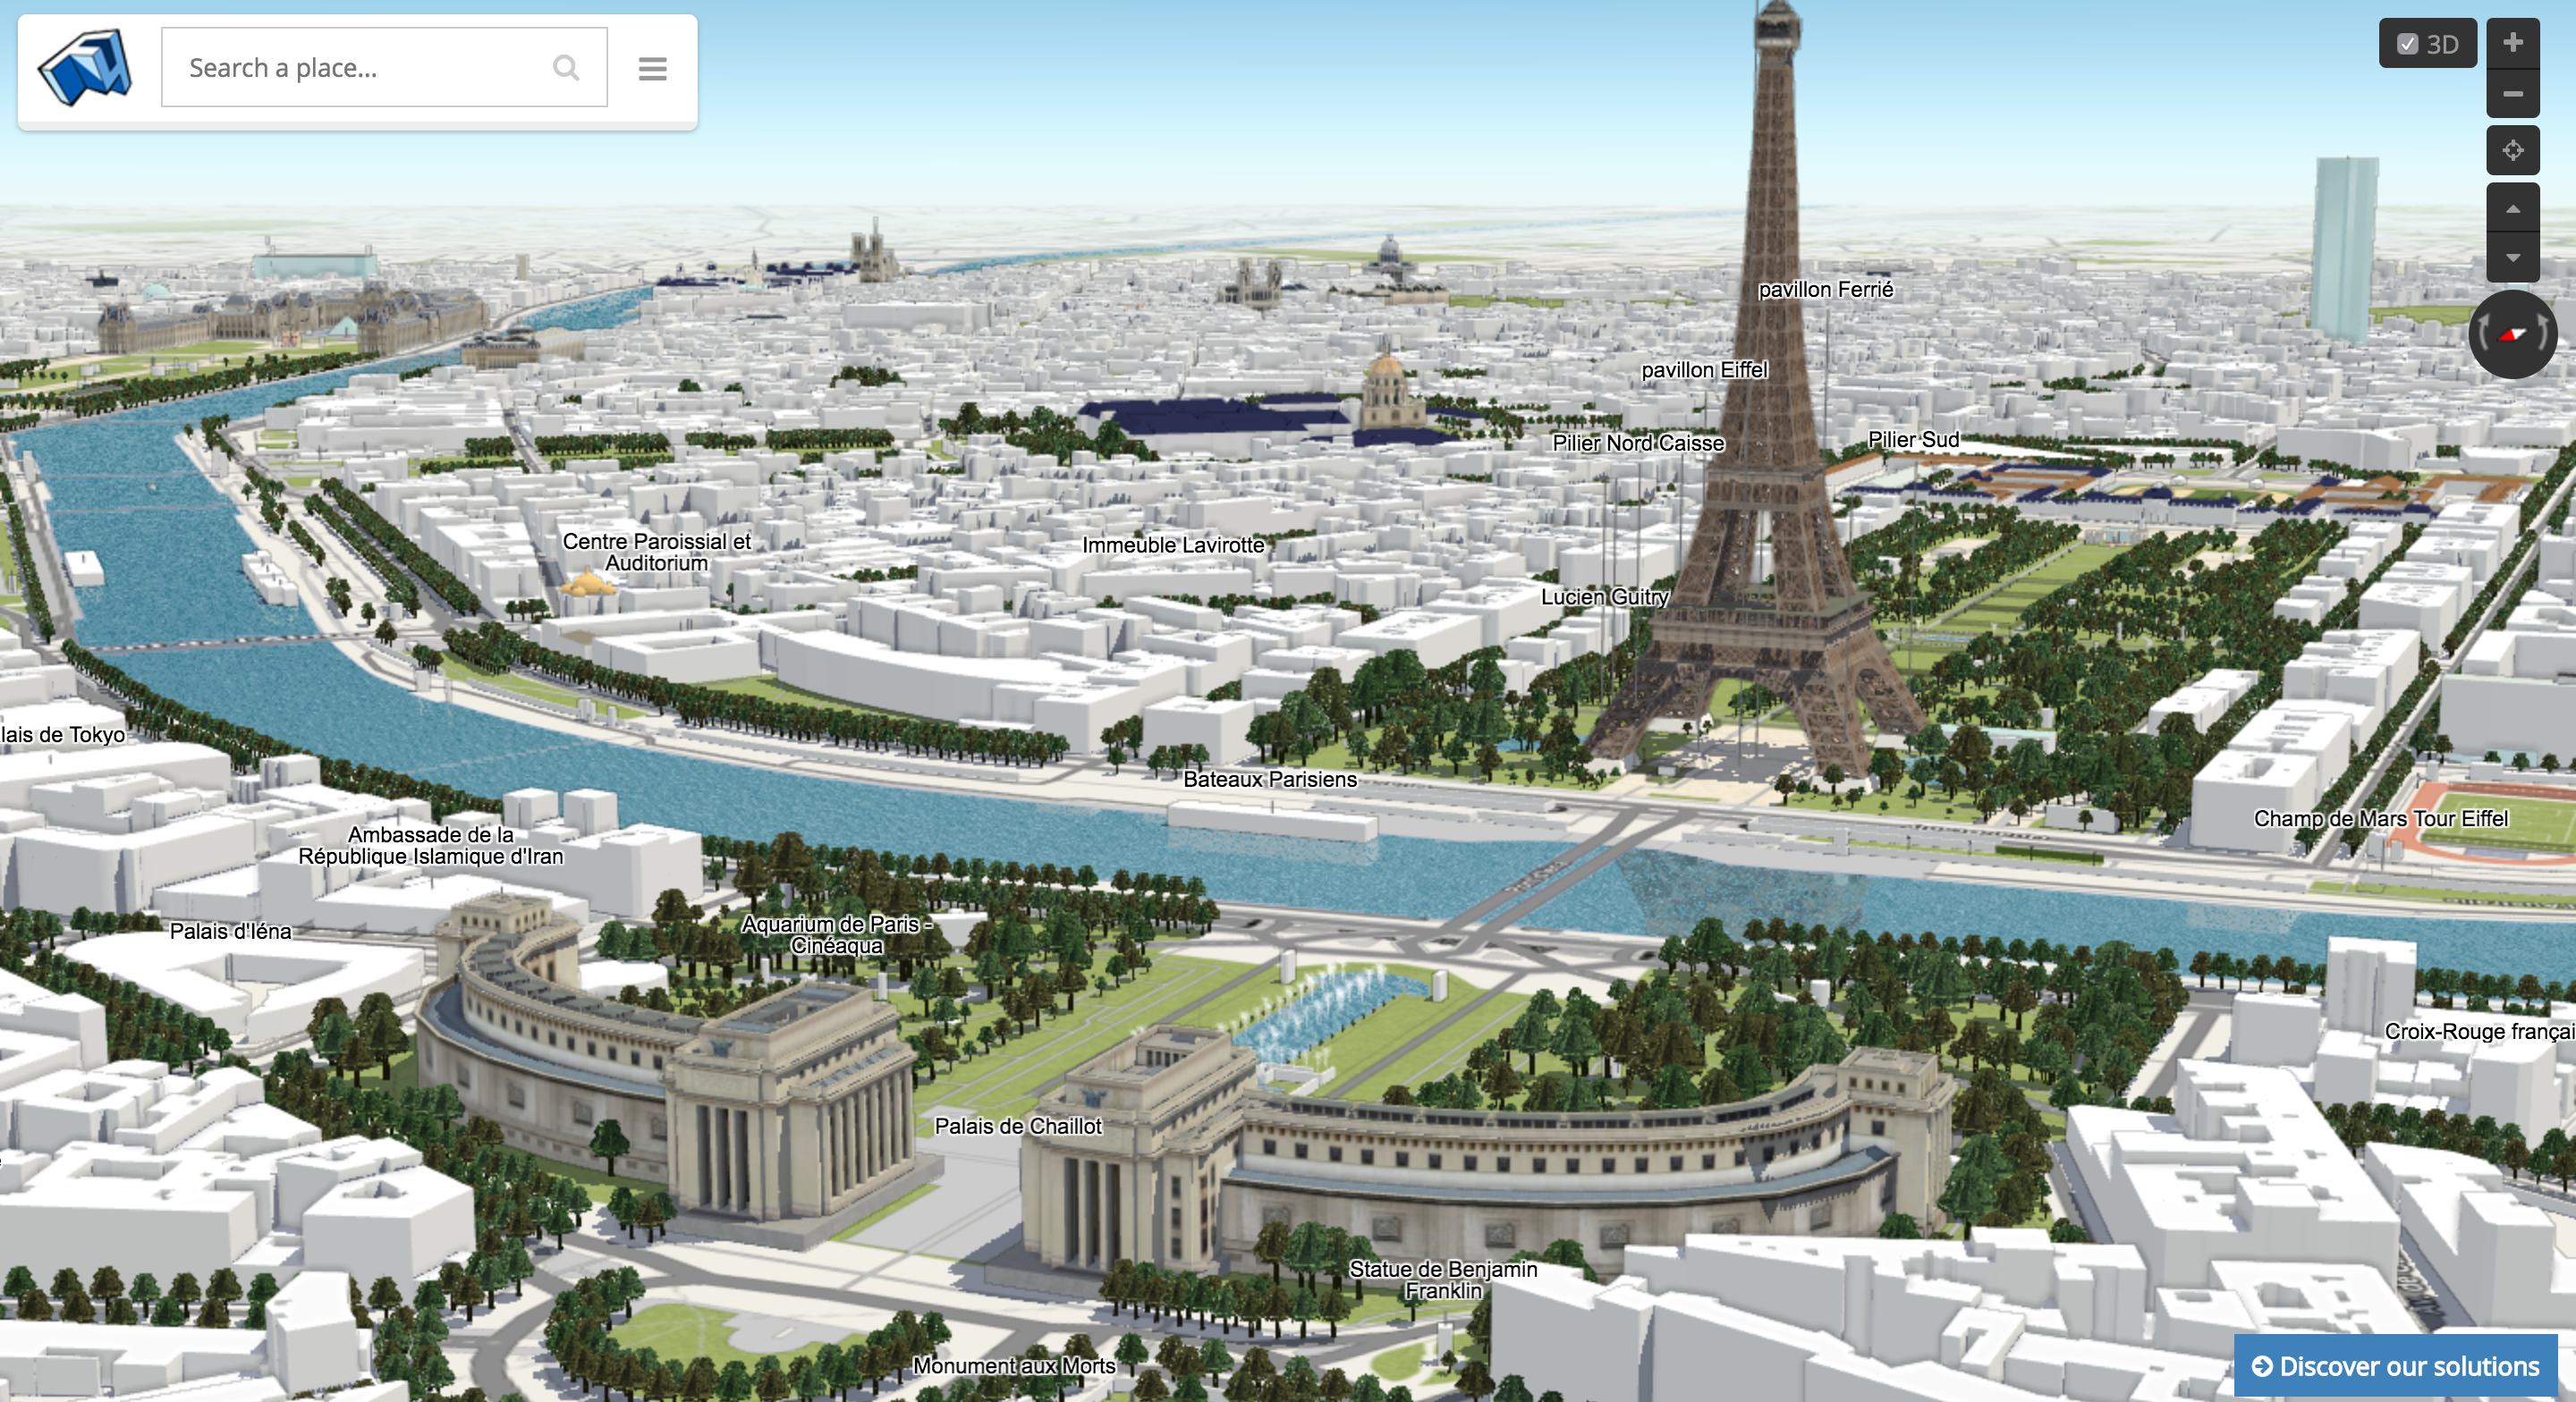
\includegraphics[width=0.8\textwidth]{chapter2/images/F4-Map}
\caption{A visualization of Paris using F4 Map}
\label{fig:F4-Map}
\end{figure}
Unfortunately, the F4 group does not provide any kind of documentation and this project is not open source.
\subsubsection{ViziCities}
The third and last map that uses OSM information about buildings is ViziCities, a framework for 3D geospatial visualization in the browser. It's code is available on GitHub since it is an OpenSource project but they are still at version 0.3 of the application.\\It let the developer add some useful information to the map like routes and GeoJSON (i.e., a format for encoding a variety of geographic data structures) but is still very limited and not very prone to interactivity.
\begin{figure}[H]
\centering
\includegraphics[width=0.8\textwidth]{chapter2/images/vizicities-Map}
\caption{A visualization of New York city using ViziCities}
\label{fig:vizicities-Map}
\end{figure}

\subsection{Cesium}
\begin{figure} [h]
\centering
\includegraphics[width=0.4\textwidth]{chapter2/images/cesium_logo}
\caption{Cesium logo}
\label{fig:cesium_logo}
\end{figure}
Cesium is an open-source JavaScript library for world-class 3D globes and maps that is used to create a web-based globe and map for visualizing dynamic data. This framework runs using WebGL, a JavaScript API for rendering 3D graphics within any compatible web browser that allows GPU--accelerated usage of physics and image processing and effects as part of the web page canvas.\\ 
The features that Cesium provides are the following:
\begin{itemize}
	\item {\bf A virtual globe:} a three-dimensional software model or representation of the Earth that provides the user with the ability to freely move around in the virtual environment by changing the viewing angle and position.
	\item {\bf Different imagery providers:} the possibility to draw and layer high-resolution imagery (maps) from several standard services directly on the virtual globe. 
	\begin{figure} [h]
		\centering
		\begin{subfigure}[b]{0.3\textwidth}
			\includegraphics[width=1\textwidth]{chapter2/images/Bing-Map}
			\caption{High-resolution, mesh-based terrain provided by Bing}
			\label{fig:Bing-Map}
		\end{subfigure}
		 \qquad
		\begin{subfigure}[b]{0.3\textwidth}
			\includegraphics[width=0.993\textwidth]{chapter2/images/Mapbox-Map}
			\caption{Streets basic imagery provided by Mapbox}
			\label{fig:Mapbox-Map}
		\end{subfigure}
		\caption{Example of two imagery providers available on Cesium}
	\end{figure}

	\item {\bf Different terrain providers:} the possibility to visualize global high-resolution terrain and water effects for oceans, lakes, and rivers but mostly the possibility to represent mountain peaks, valleys, and other terrain features. 
	\begin{figure} [H]
		\centering
		\begin{subfigure}[b]{0.3\textwidth}
			\includegraphics[width=1\textwidth]{chapter2/images/2D-Map}
			\caption{The standard WGS84 Ellipsoid}
			\label{fig:2D-Map}
		\end{subfigure}
		 \qquad
		\begin{subfigure}[b]{0.3\textwidth}
			\includegraphics[width=0.993\textwidth]{chapter2/images/3D-Map}
			\caption{Terrain meshes provided by STK}
			\label{fig:3D-Map}
		\end{subfigure}
		\caption{Example of two terrain providers available on Cesium, this shows the benefits of a 3D globe compared to a 2D map.}
	\end{figure}
	\item {\bf Huge number of API provided:} since the uses of Cesium are really various, Cesium provides a very big number of API in order to control every aspect of the web application (i.e., draw every kind of geometry, handle animations, etc\dots).\\The official website of Cesium, also provides a complete documentation, various examples and playgrounds.
\end{itemize}

\begin{figure} [H]
\centering
\includegraphics[width=0.9\textwidth]{chapter2/images/NewYorkCityCesium3dTiles}
\caption{An example showing a 3D visualization of the city of New York. Using Cesium 3D Tiles Tecnhology}
\label{fig:NewYorkCityCesium3dTiles}
\end{figure}
\subsection{Swiss Geospatial Portal Using 3D Tiles}
\begin{figure} [H]
\centering
\includegraphics[width=0.9\textwidth]{chapter2/images/BernCitySwissTopo}
\caption{A 3D visualization of the city of Bern in the Swiss Geospatial Portal. Using Cesium 3D Tiles Tecnhology}
\label{fig:BernCitySwissTopo}
\end{figure}
%%%%%%%%%%%%%%%%%%%%%%%%%
%%%%%%%%%%%%%%%%%%%%%%%%%
\section{\applicationName} \label{projectDesign}
%%%%%%%%%%%%%%%%%%%%%%%%%
\subsection{Environment and Frameworks}
The environments selected to develop \applicationName\ are the following:
\begin{itemize}
	\item {\bf The Server--side} was written using the {\bf Java} Programming Language. The {\bf Spring Framework} was used, in particular using its most famous convention--over--configuration, called {\bf Spring Boot}. The database used to store the information about the city is {\bf MySQL}.
	\item {\bf The Client--side} was written using the {\bf Javascript} scripting language. The {\bf jQuery} library was used and, of course, {\bf HTML5} and {\bf CSS3}. As mentioned above, the 3D visualization of the city was achieved using the {\bf Cesium Framework}
\end{itemize}

\subsection{The Overall Structure}

\subsection{Server Side}
\subsubsection{Models}
\subsubsection{Parser}
\subsubsection{Cron Jobs}
\subsubsection{Controllers}
\subsection{Client Side}
\subsubsection{The first Attempt: Babylon.js}
Immediately after having gathered the essential data useful to draw the buildings of the city of Lugano, a first attempt of visualizing them was made using BabylonJS. It is a JavaScript framework for building 3D environments with HTML5 and WebGL. It allows the creation of a scene with customized lights, cameras, materials, meshes, animations, audio and actions. It also supports scene picking (i.e., an element on the scene is clickable and it is possible to interact with it).\\

In order to test the capabilities of BabylonJS, a small portion of Lugano (i.e., the part around the lake) was selected and rendered. The result can be seen in the following image:
\begin{figure}[H]
\centering
\includegraphics[width=0.8\textwidth]{chapter3/images/babylonJS}
\caption{The first attempt of city visualization using BabilonJS}
\label{fig:babilonJS}
\end{figure}
As long as the buildings showed in the scene where under the two--thousand, the browser was very fast in rendering during the loading of the page and the movement of the camera was smooth.\\
The main problems that make the idea to use BabylonJS discarded, were has been basically two:
\begin{itemize}
	\item The buildings to be rendered were far above the mentioned threshold, the rendering would take more than 30 seconds.
	\item BabylonJS provides no basis to start from: the initial scene is completely empty and, as it is possible to see in the image above, buildings lay on a plane. That represented a serious problem since the visualization of the city was planned to be shown in a way that would be as realistic as possible.
\end{itemize}
A solution to the last problem would have been using the Google Elevation API. This service, given a pair of coordinates (i.e., latitude and longitude), returns the exact altitude of that point.\\

Unfortunately, the API system of Google provides just 2,500 free requests per day. In the case of Lugano, that extends its territory for more that $25km^2$, considering one request for meter it would have been taken more than 10 days to get the entire terrain structure (for the entire city of Rome, that spans almost $46km^2$, the days taken would have been more than 20).\\

Nonetheless, this would have made the rendering slower since, in addition to the visualization of the buildings, also a rendering of the terrain (i.e., lakes, mountains and rivers) would have taken place.\\
Therefore, this lack of both Google--API--requests and good performances, lead the idea to use BabylonJS to be discarded.
\subsubsection{The final version: Cesium.js}
As stated above, the Cesium Framework was finally used to build the client--side of the application.\\
Cesium, on the contrary, provides a ready--to--use virtual globe
\subsubsection{The Side Menu and The Query Builder}
\subsubsection{Cesium Framework}
%%%%%%%%%%%%%%%%%%%%%%%%%
%%%%%%%%%%%%%%%%%%%%%%%%%
\section{Use Cases} \label{useCases}
%%%%%%%%%%%%%%%%%%%%%%%%%
In this chapter some of the possible actions that can be performed into \applicationName\ are presented. The aim of this chapter is to provide a practical introduction to \applicationName, through different use cases.
\subsection{Access information}
The first use case presented introduces the available option to access building models data.\\
An InfoBox is shown, whenever a building is selected through a click of the mouse or a tap on the screen of a smartphone. Figure \ref{subfig:infoBox} and Figure \ref{subfig:infoBox_city} shows how these information are given to the user.\\
\begin{figure} [h]
\centering
	\includegraphics[width=0.8\textwidth]{chapter4/images/infoBox_city}
	\caption{Selecting a building will make the InfoBox appear automatically}
	\label{subfig:infoBox_city}
	\end{figure}
\begin{figure} [h]
	\centering
	\includegraphics[width=0.5\textwidth]{chapter4/images/infoBox}
	\caption{A detailed look at the InfoBox}
	\label{subfig:infoBox}
\end{figure}
The first field displayed is a 3D representation of the model of the building clicked without its surrounding environment. It is possible to interact with this canvas in order to rotate and zoom the building model freely.\\
After, a list of useful information about the building follows: the length of this list changes from building to building depending on the availability of the information.\\
The building clicked in the example of figure \ref{fig:infoBox} presents all the possible available information that an user can get about a building.\\
The fields of the displayed data are denoted as follows: 
\begin{itemize}
\item {\bf Types} provides the list of groups in which the building is present. Groups are defined by the OpenStreetMap APIs and are used to represent the usage of the buildings which, conceptually, have characteristics in common. Examples of types are: Post Office, Pharmacy, Hospital, University etc \dots.
\item {\bf Floors} is the number of floors that the building possesses
\item {\bf Shape Length \& Shape Area} represent the size of buildings available for consultancy, they are measured in length and area both expressed in meters.
\item {\bf Street Name \& Civic Numbers} are the data concerning the addresses of the street where the building is located. There could be more than one street name and civic numbers in case the building has many of them (e.g., different entrances in the same building that are on different streets). Addresses data are taken from Swisstopo APIs and, if not available from this service, OpenStreetMap APIs are used.
\item {\bf EGID} the unique identifier of the building given by the Swiss REA 
\item {\bf Suburb} represents the suburb in which the building is located
\item {\bf Primary \& Secondary houses} represents both the number of primary and secondary houses in the selected building and the percentage that each value represents over the total number of houses in that building
\end{itemize}

\subsection{Visualize the City}
The first tab available to the user when the side--bar is opened, is the Visualize Tab. It is divided into three main subsections: ``Show on the map'', ``Color city'' and ``Show Suburbs''.\\

The first subsection contains two checkboxes: the first one, let the user show the geolocalization, i.e., the position of the device from which the user is using \applicationName. The second checkbox, if checked, shows the position of webcams located around Lugano; this webcams continuously stream videos of the city. In Figure \ref{fig:mapPins} it is possible to see the result on the map, when both checkboxes are checked.
\begin{figure} [H]
\centering
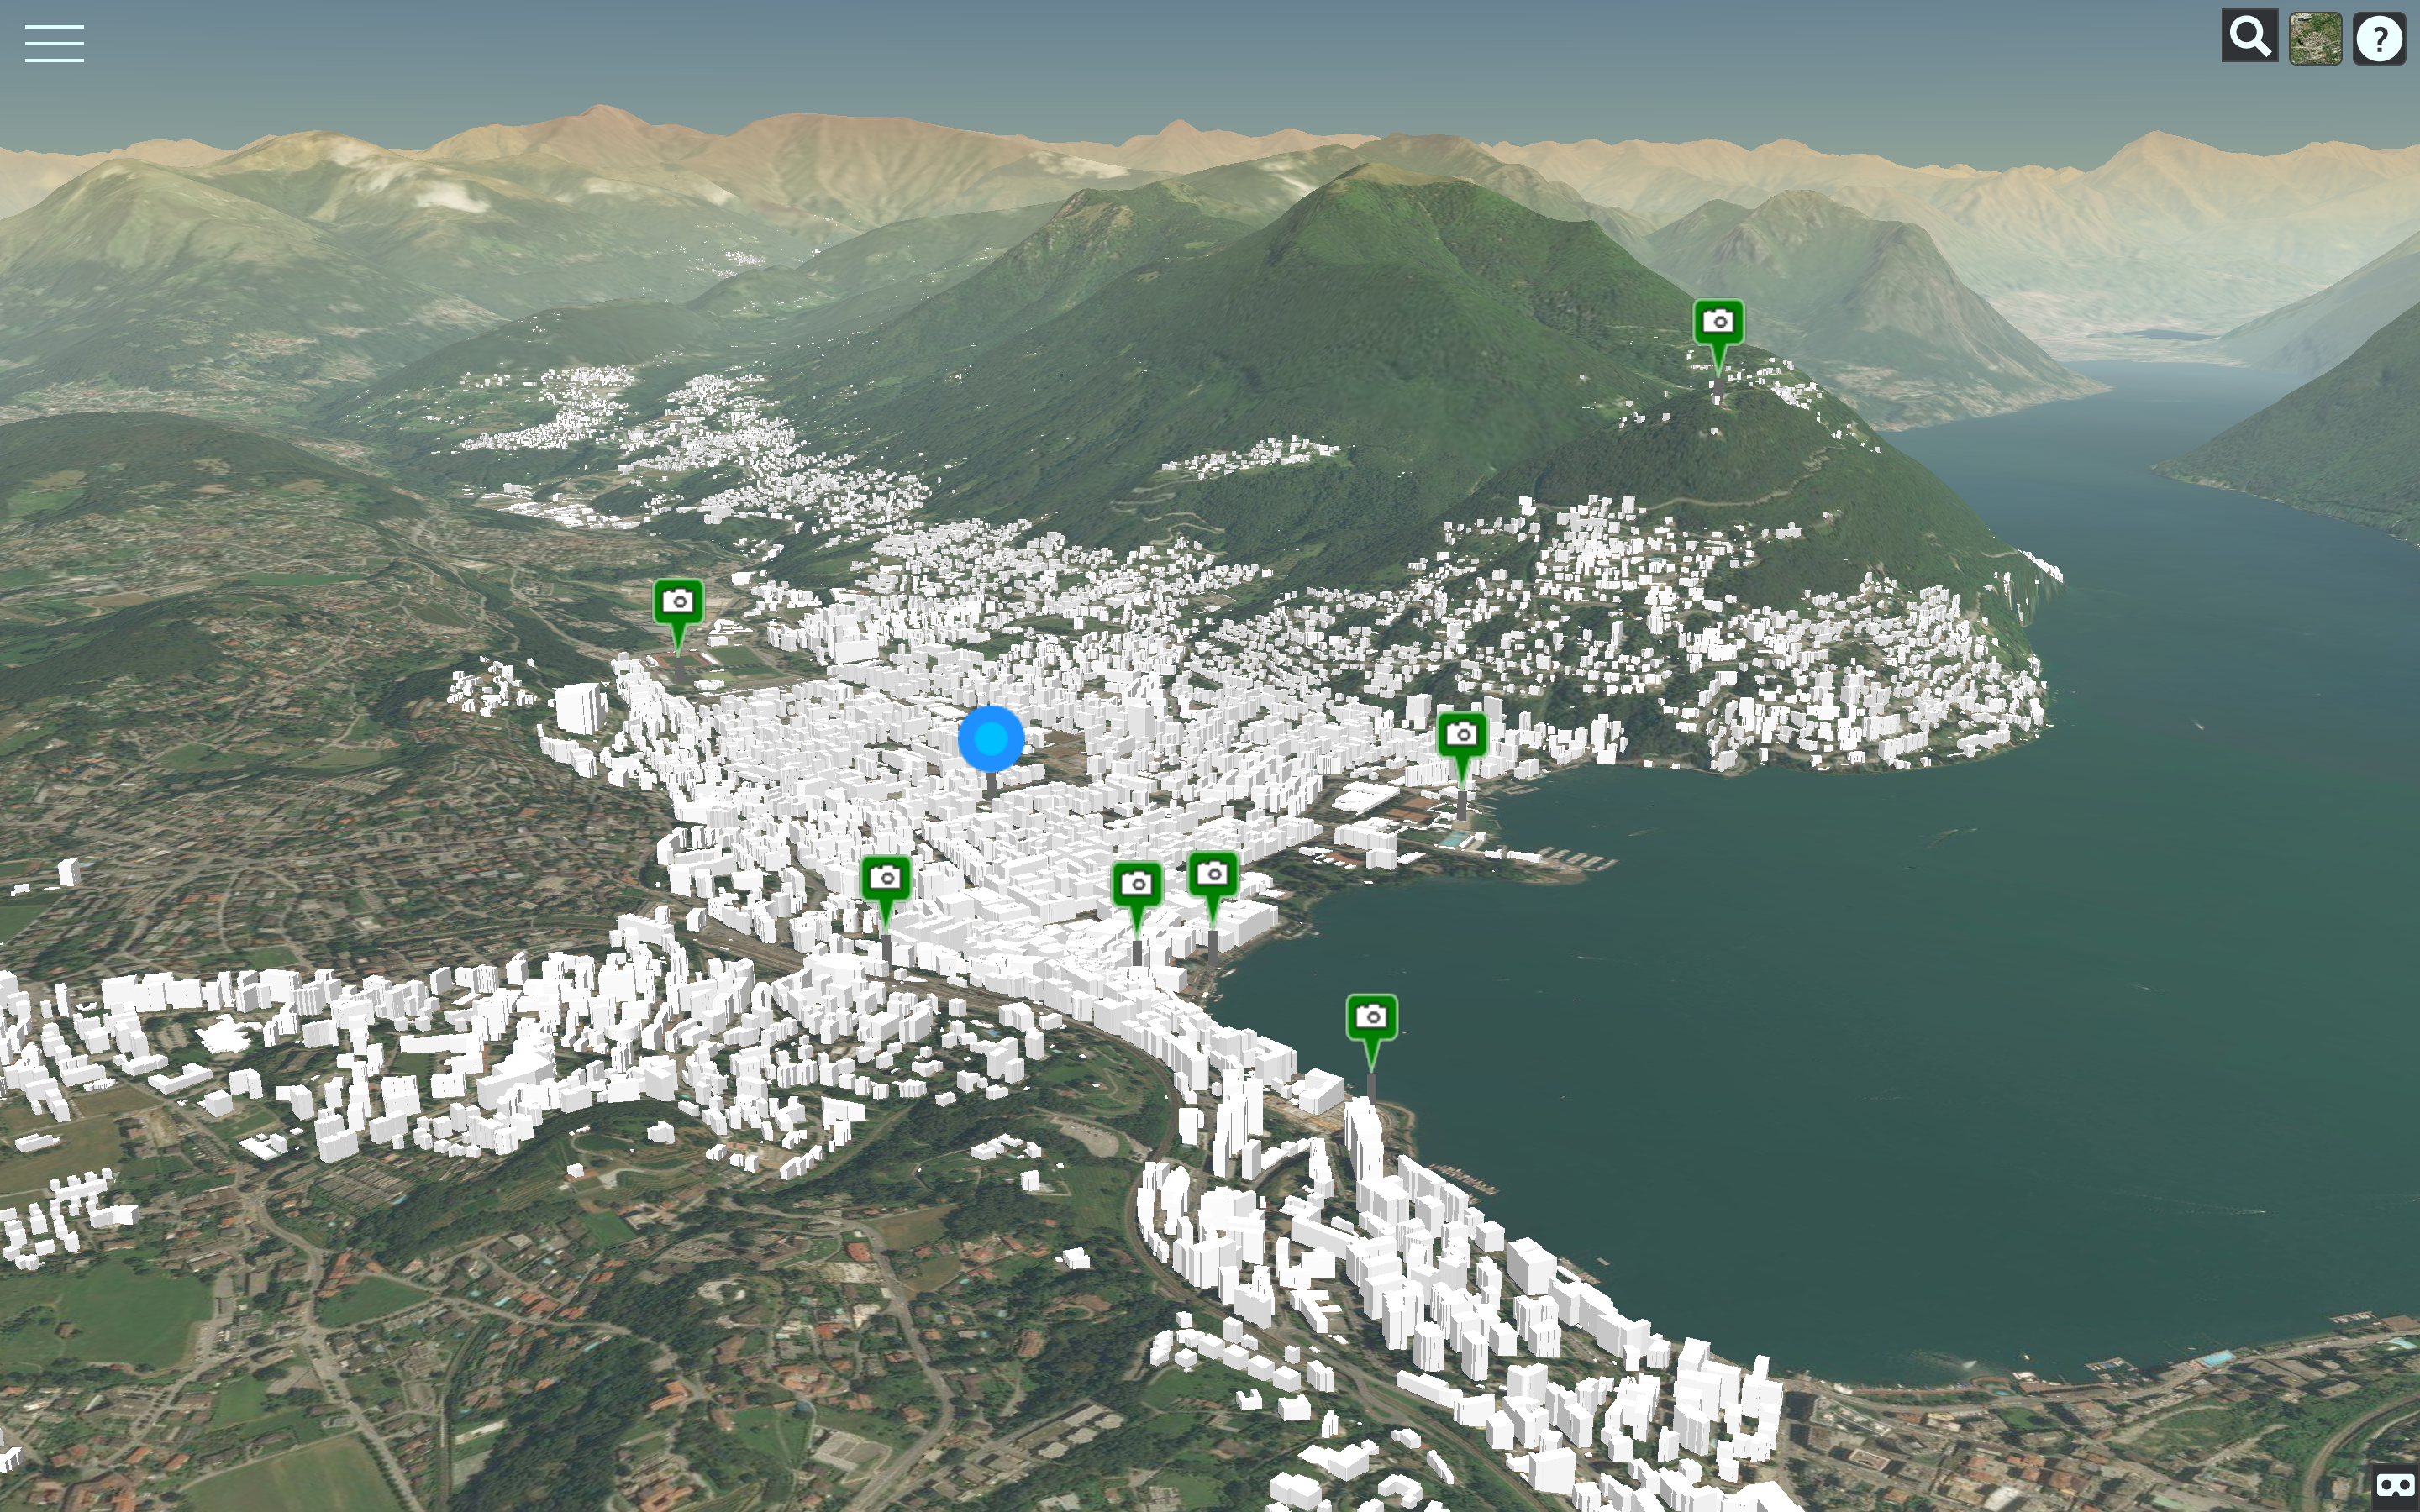
\includegraphics[width=.8\textwidth]{chapter4/images/mapPins}
\caption{When both checkboxes are checked, geolocalization and webCams positions are shown on the map}
\label{fig:mapPins}
\end{figure}
Since the 3D visualization had still to allow the user to exactly locate the position of these pins, whenever the visualization is more zoomed it it, a ``stick'' is created starting from the ground and ending at the bottom of the pin, as it is shown in Figure \ref{fig:3dPins}.\\

\begin{figure} [H]
\centering
\includegraphics[width=.8\textwidth]{chapter4/images/3dPins}
\caption{The ``Stick'' that connects the ground to the pins}
\label{fig:3dPins}
\end{figure}
In the second subsection three radio buttons can be found: the first one is used to reset the color of the entire city to the default color. The second colours the buildings in the city based on their height (Figure\ref{fig:application_byHeight}). The third one is used to colour the entire city based on its suburbs and so every suburb has a different color(Figure \ref{fig:application_showSuburb} ).\\

\begin{figure} [H]
\centering
\includegraphics[width=.8\textwidth]{chapter4/images/application_bySuburb}
\caption{A Visualization of the city of Lugano where every suburb is coloured differentrly}
\label{fig:application_bySuburb}
\end{figure}
\begin{figure} [H]
\centering
\includegraphics[width=.8\textwidth]{chapter4/images/application_byHeight}
\caption{A Visualization of the city of Lugano where every building is colorued based on its height}
\label{fig:application_byHeight}
\end{figure}
The third and last subsection, contains the list of checkboxes representing all the suburbs in the city and their respective colours. By default all checkboxes are checked but uncheck them will result in hiding the desired suburb as show in Figure \ref{fig:application_showSuburb}.
\begin{figure} [H]
\centering
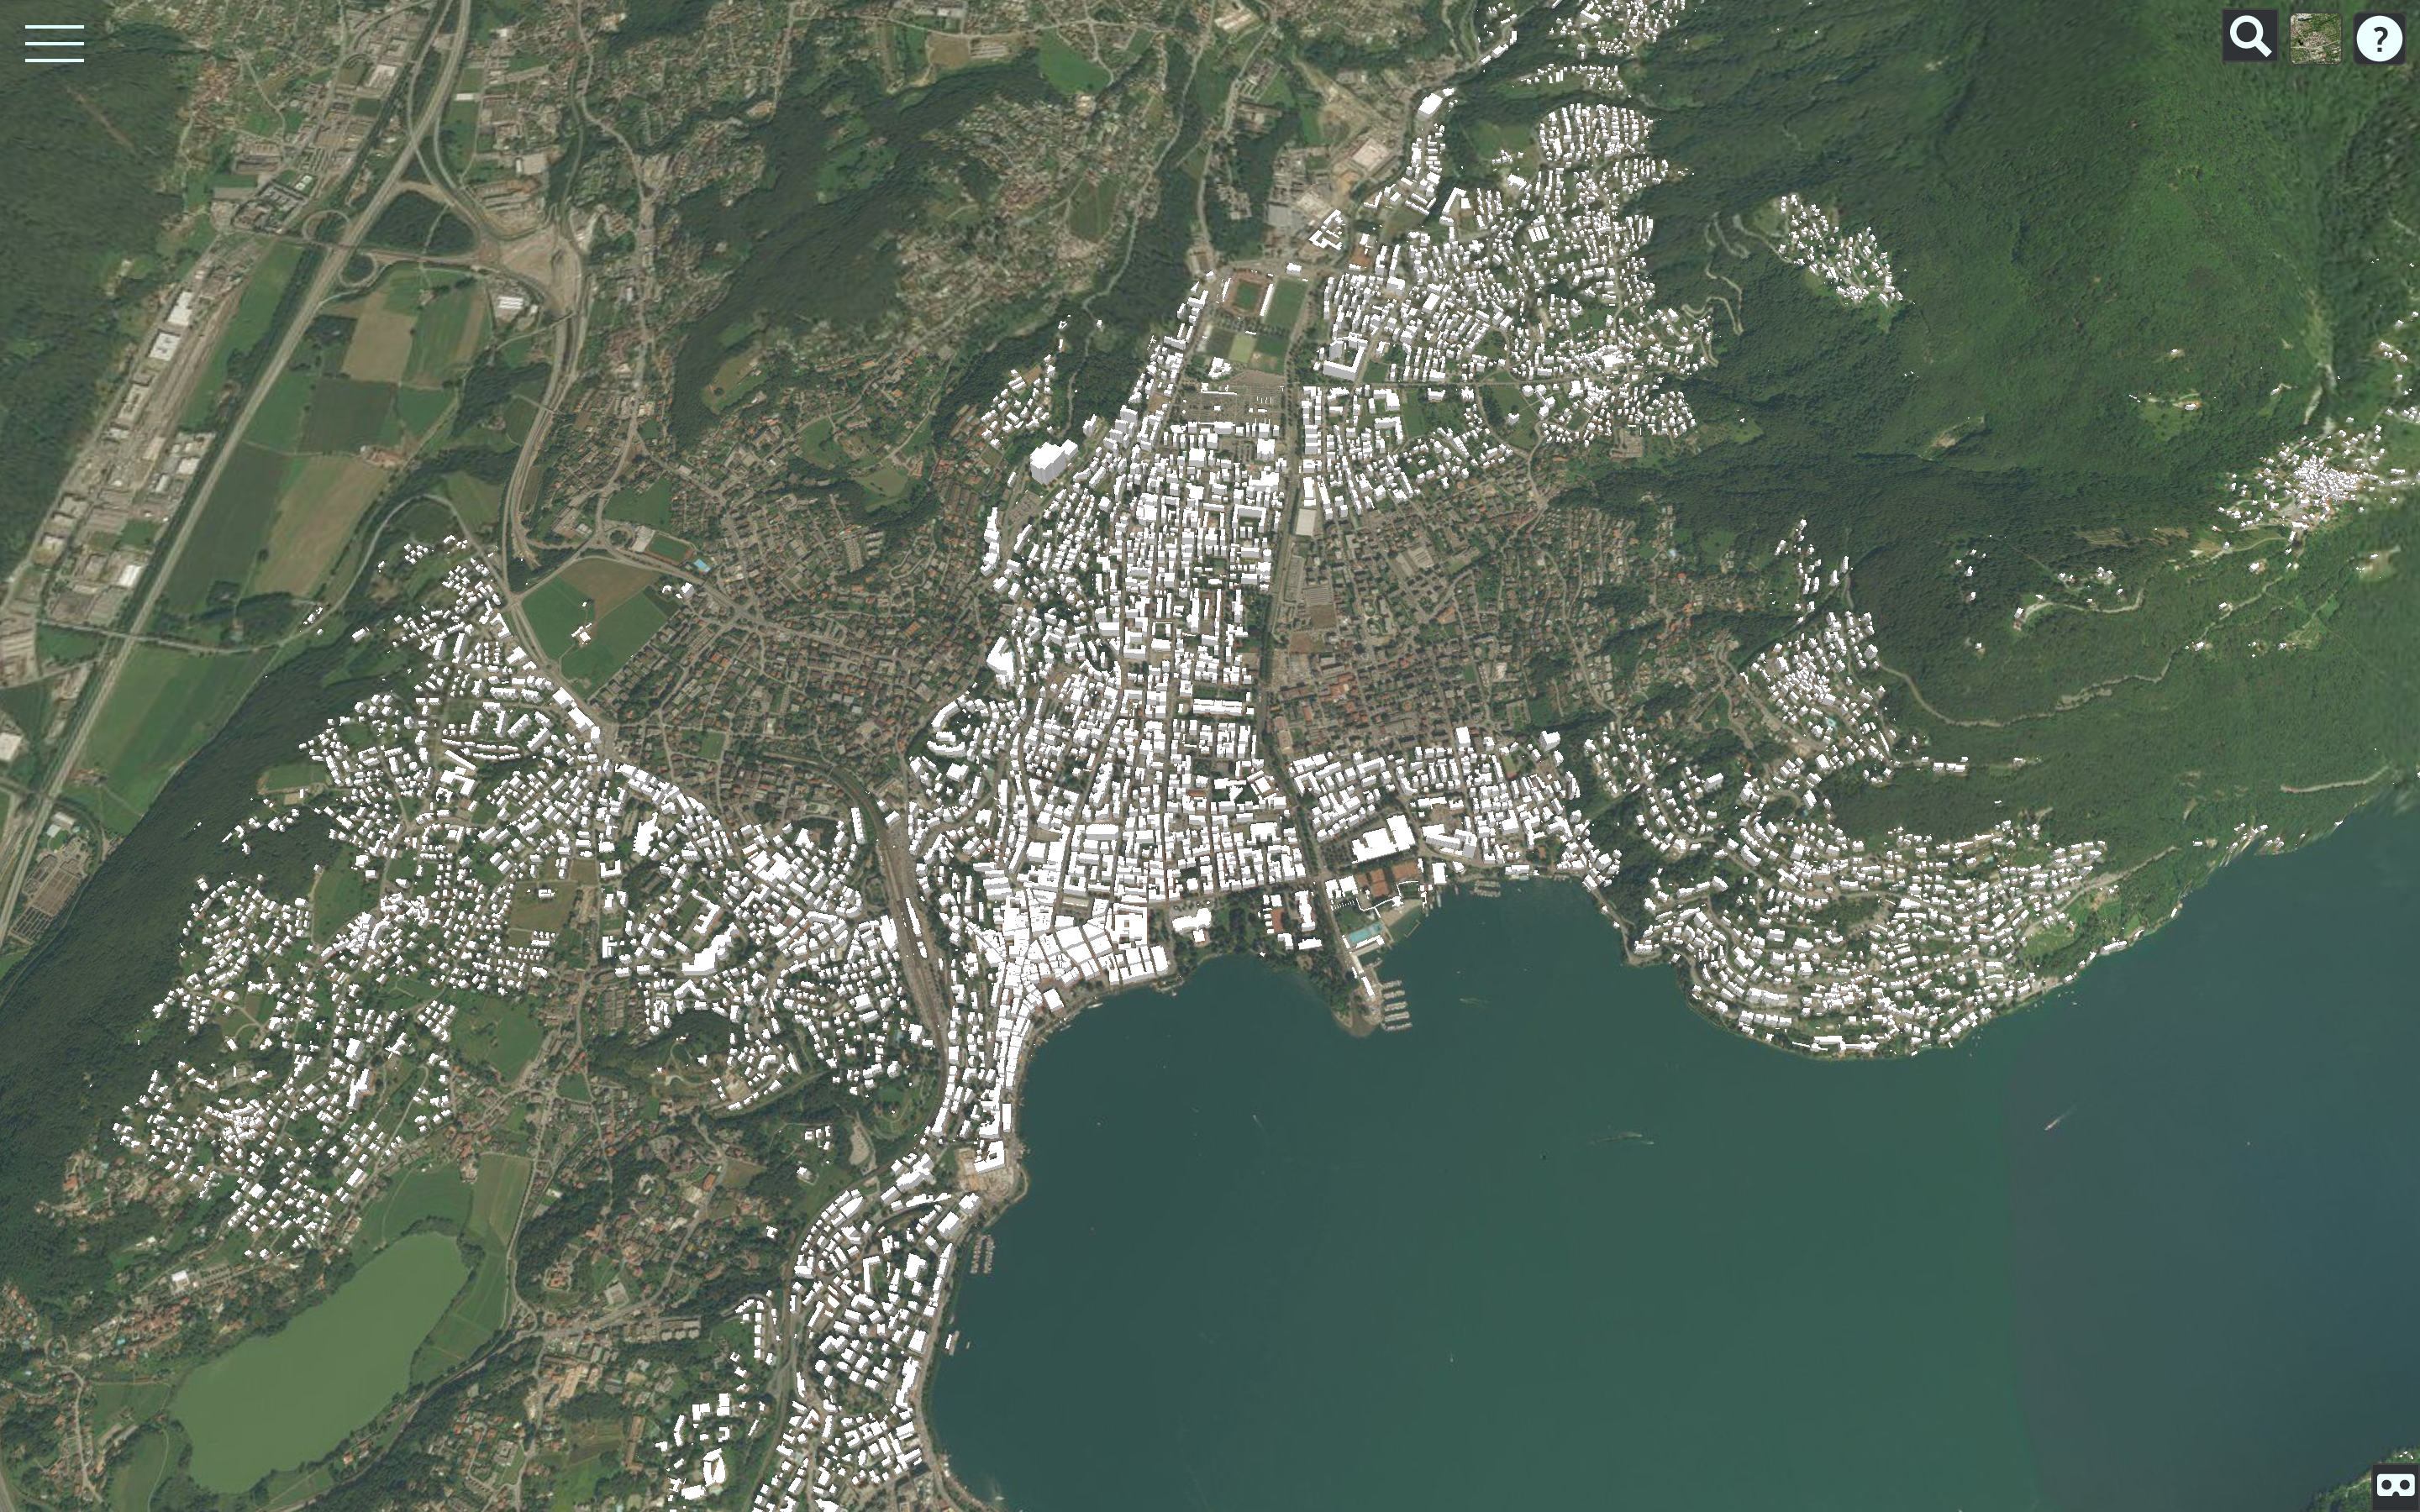
\includegraphics[width=.8\textwidth]{chapter4/images/application_showSuburb}
\caption{A Visualization of the city of Lugano where the suburb Viganello is hidden}
\label{fig:application_showSuburb}
\end{figure}

\subsection{The Query System}
\subsubsection{Building Selection}
This use case shows what actions can be performed using the visual query system. The interactions proposed are accessible through the apposite ``Query City'' selection tab in the provided sidebar.\\
As it is possible to see on Figure \ref{fig:query_city_tab} in the previous chapter, \applicationName\ allows the user to perform from very single to more complex query on the entire city.
\subsubsection{City Gradient Map}
%%%%%%%%%%%%%%%%%%%%%%%%%
%%%%%%%%%%%%%%%%%%%%%%%%%
\section{Conclusion} \label{conclusions}
%%%%%%%%%%%%%%%%%%%%%%%%%
\subsection{Potential and Limits}
In our opinion the tool has great potential. As explained above, even if there are many tools which represent cities in 3D, very few of them are able to allow interactions and almost none of them allow the possibility to do query like presented in \applicationName. We think that the possibility to take plain alphanumeric data and gives it a virtual representation which provides visual feedback is the success key of this application.\\

The main limits of \applicationName\ are the lack of additional data about the urban environment (e.g., traffic data) and the quality of data provided by third party entities (e.g., OpenStreetMap). We did not manage to always find accurate data to inject in the example of Lugano, therefore we were limited to make interactions with the available data. Since not all data was available for each building, where data was missing we had to fill in with OpenStreetMap's information that were not always accurate.

\subsection{Future Work or Possible Developments}
Right now \applicationName is a prototype which could be further developed, since the ways out of this application are really limitless. With some more data available like a more accurate representation of the buildings, it could be possible to result in an even nicer and more precise 3D--visualization. In addition, more information related to buildings, bus stops, actual streets, rivers, bridges, green zones and tunnels could be included. Once other elements are available in the representation further interactions could be implemented raising the level of visual feedback provided by the tool.\\

\applicationName, with its graphical rapresentation and interactivity, has raised interest in both private citizens and the public sector. The City of Lugano stated interest on the potential application of \applicationName, and suggested a novel visualization on data that involves primary and secondary residence.\\

Our future work involves integration with better data sources, like Google Maps. We also plan to integrate more refined 3D models of buildings as provided by Swisstopo.

%%%%%%%%%%%%%%%%%%%%%%%%%

%\begin{table}[h]
%\centering
%\scalebox {0.8} {
%\begin{normalsize}\begin{tabular}{l|lll}
%\textbf{Col 1} & \textbf{Col 2} & \textbf{Col 3} & \textbf{Col 4}\\
%\hline
%1 & 2 & 3 & Goofy\\
%4 & 5 & 6 & Mickey
%\end{tabular}
%\end{normalsize}
%}
%\caption{Caption of the table}
%\label{tab:numbers}
%\end{table}

%\cite{Stru1899a}
%%%%%
%\newpage
%\bibliographystyle{abbrv}
%\bibliography{references}

\end{document}